\chapter{Classification Accuracy}
\label{ch:classification_accuracy}

Now that we know what classification trees are, the next question is what is the quality of their predictions. For beginning, we need to define what we mean by quality. In classification, the simplest measure of quality is classification \marginnote{$\mathrm{accuracy}=\frac{\# \{\mathrm{correct}\}}{\# \{\mathrm{all}\}}$} accuracy expressed as the proportion of data instances for which the classifier correctly guessed the value of the class. Let's see if we can estimate, or at least get a feeling for, classification accuracy with the widgets we already know.

\begin{wrapfigure}{o}{0.85\textwidth}
    \vspace{-0.5cm}
    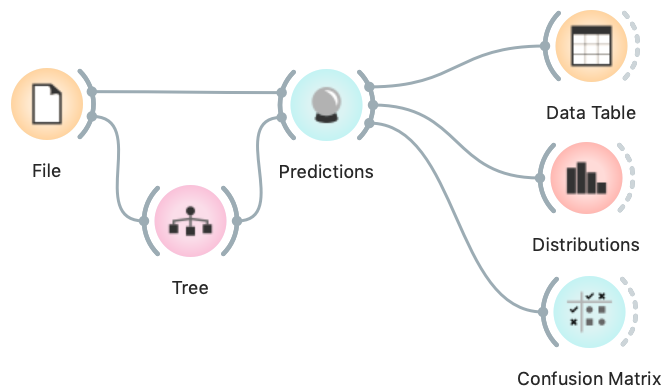
\includegraphics[scale=0.35]{workflow.png}
\end{wrapfigure}

Let us try this schema with the \textit{iris} data set. The \widget{Predictions} widget outputs a data table augmented with a column that includes predictions. In the \widget{Data Table} widget, we can sort the data by any of these two columns, and manually select data instances where the values of these two features are different (this would not work on big data). Roughly, visually estimating the accuracy of predictions is straightforward in the \widget{Distribution} widget, if we set the features in view appropriately.

For precise statistics of correctly and incorrectly classified examples open the \widget{Confusion Matrix} widget.

\begin{figure*}[h]
    \centering
    \newcommand{\predictions}{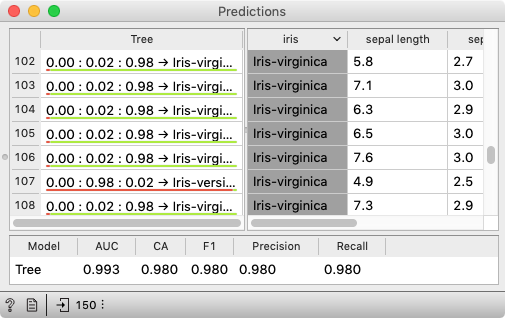
\includegraphics[scale=0.40]{predictions2.png}}
    \newcommand{\distributions}{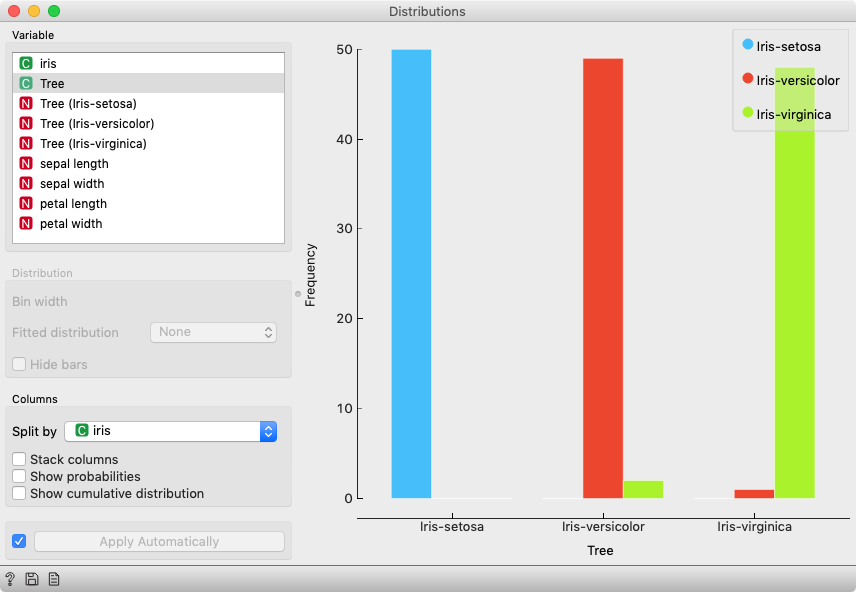
\includegraphics[scale=0.25]{distributions.png}}
    \newcommand{\confusion}{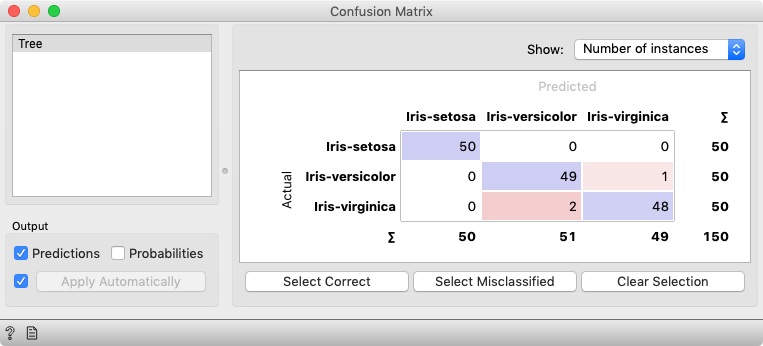
\includegraphics[scale=0.25]{confusion.png}}
    \infinitewidthbox{
    \stackinset{r}{-0.35\linewidth}{b}{-0.05\linewidth}{\confusion}
    {\stackinset{r}{-0.35\linewidth}{b}{+0.15\linewidth}{\distributions}{\predictions}}\hspace{7cm}
    }
    \caption{The \widget{Confusion Matrix} shows 3 incorrectly classified examples, which makes the accuracy $(150-3)/150 = 98\%$.}
\end{figure*}
